% !TEX TS-program = pdflatex
% !TEX encoding = UTF-8 Unicode

% This is a simple template for a LaTeX document using the "article" class.
% See "book", "report", "letter" for other types of document.

\documentclass[11pt]{scrartcl} % use larger type; default would be 10pt

\usepackage[utf8]{inputenc} % set input encoding (not needed with XeLaTeX)

%%% Examples of Article customizations
% These packages are optional, depending whether you want the features they provide.
% See the LaTeX Companion or other references for full information.

%%% PAGE DIMENSIONS
\usepackage{geometry} % to change the page dimensions
\geometry{a4paper} % or letterpaper (US) or a5paper or....
% \geometry{margin=2in} % for example, change the margins to 2 inches all round
% \geometry{landscape} % set up the page for landscape
%   read geometry.pdf for detailed page layout information

\usepackage{graphicx} % support the \includegraphics command and options

% \usepackage[parfill]{parskip} % Activate to begin paragraphs with an empty line rather than an indent

%%% PACKAGES
\usepackage{booktabs} % for much better looking tables
\usepackage{array} % for better arrays (eg matrices) in maths
\usepackage{paralist} % very flexible & customisable lists (eg. enumerate/itemize, etc.)
\usepackage{verbatim} % adds environment for commenting out blocks of text & for better verbatim
\usepackage{subfig} % make it possible to include more than one captioned figure/table in a single float
\usepackage{graphicx}
% These packages are all incorporated in the memoir class to one degree or another...
\usepackage{hyperref}

%%% SECTION TITLE APPEARANCE
\usepackage{sectsty}
\allsectionsfont{\sffamily\mdseries\upshape} % (See the fntguide.pdf for font help)
% (This matches ConTeXt defaults)

%%% ToC (table of contents) APPEARANCE
\usepackage[nottoc,notlof,notlot]{tocbibind} % Put the bibliography in the ToC
\usepackage[titles,subfigure]{tocloft} % Alter the style of the Table of Contents
\renewcommand{\cftsecfont}{\rmfamily\mdseries\upshape}
\renewcommand{\cftsecpagefont}{\rmfamily\mdseries\upshape} % No bold!


\usepackage{amssymb}
\usepackage{amsmath}
\usepackage{mathcomp}
%\usepackage{colortbl}
\usepackage{dsfont}
\usepackage{amsfonts}
\usepackage{cancel}

%%% KV-Diagramme
%\usepackage[ngerman]{babel}
\input kvmacros

%%% Graphen
\usepackage{tikz}
\usetikzlibrary{intersections}
\usetikzlibrary{calc}

% last page
\usepackage{pageslts}

%%% END Article customizations

%%% HEADERS & FOOTERS
\usepackage{fancyhdr} % This should be set AFTER setting up the page geometry
%\usepackage{scrpage2} % Another package (only use fancyhdr or scrpage2)
\pagestyle{fancy} % options: empty , plain , fancy
\renewcommand{\headrulewidth}{1.2pt} % customise the layout...
\renewcommand{\footrulewidth}{0.1pt} % customise the layout...
\lhead{MACHINE LEARNING 1\\Andres Fernandez -- 5692442 -- fr\_andres@msn.com}\chead{}\rhead{Exercise Sheet 5 \\December 5, 2016}
\lfoot{}\cfoot{\thepage/\lastpageref{LastPages}}\rfoot{}



%%% THE SYMBOLS FOR ``DEPENDENT'' AND ``INDEPENDENT''
\newcommand{\CI}{\mathrel{\text{\scalebox{1.07}{$\perp\mkern-10mu\perp$}}}} % independent
\newcommand{\nCI}{\cancel{\mathrel{\text{\scalebox{1.07}{$\perp\mkern-10mu\perp$}}}}} % dep
%% THE SYMBOL FOR DOESN'T IMPLY
\newcommand{\notimplies}{%
  \mathrel{{\ooalign{\hidewidth$\not\phantom{=}$\hidewidth\cr$\implies$}}}}

%%% The "real" document content comes below...


\begin{document}

\section*{\\[3mm]Exercise 1}
         {\it Starting from the sum-of-squares error function
           \begin{align*}
             E_D(w) = \frac{1}{2}\sum_{n=1}^N\{t_n-w^T\phi(x_n)\}^2
           \end{align*}
           derive the maximum likelihood solution for the parameters
           \begin{align*}
             w_{ML} = (\Phi^T\Phi)^{-1}\Phi^Tt
           \end{align*}
           where
           \begin{align*}
             \Phi = \begin{pmatrix}
               \phi_0(x_1) & \phi_1(x_1) & ... & \phi_{M-1}(x_1) \\
               \phi_0(x_2) & \phi_1(x_2) & ... & \phi_{M-1}(x_2) \\
               \vdots & \vdots  & \ddots & \vdots \\
               \phi_0(x_N) & \phi_1(x_N) & ... & \phi_{M-1}(x_N) \\
             \end{pmatrix}
           \end{align*}
           is the design matrix with basis functions \(\phi_j(x_i)\), \(X=\{x_1, ... x_n\}\) the vectors
           of input training data and  \(t=\{t_1, ... t_n\}\) corresponding output training
           values.
           
           
           
         }
  

         \subsection*{i)}
         A very clear and brief explanation to this topic can be found in the \href{https://github.com/dkorolev/DeepLearningBook/blob/master/DeepLearningBook.pdf}{{\it Deep Learning Book}}, page 109: Since the energy function is quadratic, the optimization solution for one dimension is convex and can be anallitically found by equalling the derivative to zero. But furthermore, a linear combination of convex optimization problems is itself convex too, since multiplication by a scalar and addition of linearly independent terms doesn't affect the outcome: the multiplicating scalars can be ignored ( In fact, the usual normalization factor \(\frac{1}{M}\) was here disregarded), and the different problems optimized separately.\\
         This is the case when performing parametric multivariate linear regression, with the \(L_2\) energy function: each weight is linearly independent from all others, and contributes to \(E\) in a convex way.
         \subsection*{ii)}
         In this terms the optimization objective can be formuled as follows:
         \begin{align*}
           \begin{aligned}
             & w_{ML} = \underset{w}{\text{minimize}}
             & & E(w, \Phi, t) = \lVert \Phi w - t \rVert_2^2 = (\Phi w - t)^T(\Phi w - t)
           \end{aligned}
         \end{align*}
         And the analytical way to find it:
         \begin{align*}
           \begin{aligned}
             \frac{\partial}{\partial w_{ML}}  E (w_{ML}, \Phi, t) = 0 \iff \frac{\partial}{\partial w_{ML}} \left((\Phi w_{ML} - t)^T(\Phi w_{ML} - t) \right) = 0\\
             \iff \frac{\partial}{\partial w_{ML}} \left(w_{ML}^T\Phi^T\Phi w_{ML} - 2w_{ML}^T\Phi^Tt+t^Tt \right) = 0\\
             \implies 2\Phi^T\Phi w_{ML} - 2w_{ML}^T\Phi^Tt = 0 \\
             \implies w_{ML} = (\Phi^T\Phi)^{-1}\Phi^Tt
           \end{aligned}
         \end{align*}
         \begin{flushright}
           $\square$\\
         \end{flushright}










         

\vspace{5mm}
\section*{Exercise 2}
         {\it Consider a data set in which each data point \((x_n, t_n)\) is associated with a weighting factor \(r_n>0\), so that the sum-of-squares error function becomes
           \begin{align*}
             E_D(w) = \frac{1}{2}\sum_{n} r_n(t_n-w^T\phi(x_n))^2
           \end{align*}
           Find an expression for the solution \(w*\) that minimizes this error function. Give two alternative interpretations of the weighted sum-of-squares error function in terms of (i) data dependent noise variance and (ii) replicated data points.}
         
         \subsection*{i)}
         The energy function can be reformulated as follows:
         \begin{align*}
           \frac{1}{2}\sum_{n} r_n(t_n-w^T\phi(x_n))^2 = \frac{1}{2}\sum_{n} {\scriptscriptstyle+}\sqrt{r_n}^2(t_n-w^T\phi(x_n))^2 \\
           = \frac{1}{2}\sum_{n} ({\scriptscriptstyle+}\sqrt{r_n}t_n-  {\scriptscriptstyle+}\sqrt{r_n}w^T\phi(x_n))^2 
         \end{align*}
         Which brings up the very same optimization objective as the one shown in Exercise 1 (assuming that the weighting factors are given and not learned, that is). Therefore, just two pre-processing calculations are needed:
         \begin{align*}
           \begin{aligned}
             t_{ML} = t\circ{\scriptscriptstyle+}\sqrt{r}\\
             \Phi_{ML} = \Phi\odot{\scriptscriptstyle+}\sqrt{r}\\
           \end{aligned}
         \end{align*}
         Whereas \({\scriptscriptstyle+}\sqrt{r}\) is the element-weise positive square root of the \(r\) vector in \(\mathbb{R}^N\), \(a\circ b\) represents the element-weise multiplication of two vectors of same dimensionality, and \(a\odot b\) abuses this notation, to represent the element-weise multiplication of each vector in the matrix a with the vector b. In This terms, the solutions is simply to apply the normal equations to the preprocessed data:
         \begin{align*}
            w_{ML} = (\Phi_{ML}^T\Phi_{ML})^{-1}\Phi_{ML}^Tt_{ML}
         \end{align*}}

         \begin{flushright}
           $\square$\\
         \end{flushright}




         \vspace{5mm}
\section*{Exercise 3}
         {\it Generate own data sets, e.g. using \(t = f(x) + 0.2\epsilon\) with \(f(x) = sin(2\pi x)\) and \(\epsilon \sim \mathcal{N}(0,1)\), and illustrate  the bias-variance decomposition by fitting a polynomial model \(y(x; w) = \sum_{i=0}^r w^ix^r\) to many different data sets \(D_1 , ... , D_L\) , each of length \(N\).\\
           Let \(w∗^D\) denote the parameters minimizing the mean squared error on dataset \(D\). Then,
           \begin{align*}
             &bias^2 \approx \frac{1}{L}\sum_l\frac{1}{N}\sum_n(\overline{y}(x)-f(x))^2\\
             &variance \approx \frac{1}{L}\sum_l\frac{1}{N}\sum_n(y(x;w*^{D_t})-\overline{y}(x)^2\\
         \end{align*}}
         where \(\overline{y}(x) = \frac{1}{L}\sum_t y(x;w*^{D_t})\)
         }


           \subsection*{Solution:}
           See/execute Python2 script{\it fernandez\_blatt5.py} for the details. As explained in the \href{http://www.ccc.cs.uni-frankfurt.de/wp-content/uploads/2016/10/week7.pdf}{{\it lecture's slides}}), the \(L_2\) loss function can be decomposed into \textbf{bias\(^2\) + variance + noise}. For a given dataset of limited size, only limited assumptions can be done: if only the variance term is taken into account (that is, no regularization term is provided), the hypothesis will maximize its adaptation to the dataset, potentially fitting perfectly to it, but it will fail to generalize, that is: to capture the underlying features. On the other side, a model excesively based on the bias term (that is, with a very high regularization index), will penalize every hypothesis that goes too far away from some given assumptions (in this case, the overall distance to the zero-vector). This assumptions may be unrealistic and relying heavily on them may be therefore a bad strategy.\\
           Both terms are based on the same input parameters, but represent opposite ideas. The bottom line behind this explanation is that a \textbf{bias-variance tradeoff} takes always place for datasets of limited size, and, unless the size of the dataset can be increased, a compromise between both of them must be achieved. This is typically achieved by testing many different regularization factors, and cross-validating the results, as shown in the Figure 1:
           \begin{figure}[ht]
	   \centering
           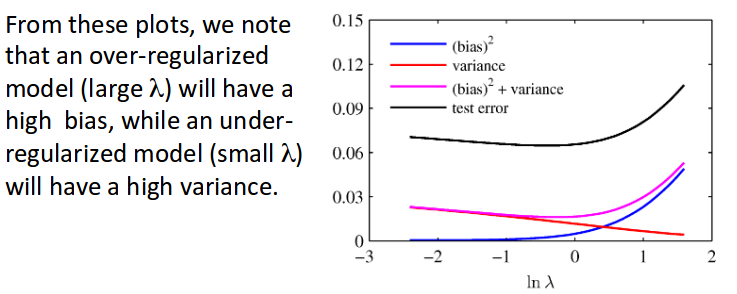
\includegraphics[width=0.8\textwidth, angle=0]{cv_reg.png}
	   \caption{test error and its decomposition for different reg. factors (lecture slides)}
	   \label{fig2}
           \end{figure}


           \begin{figure}[ht]
	   \centering
           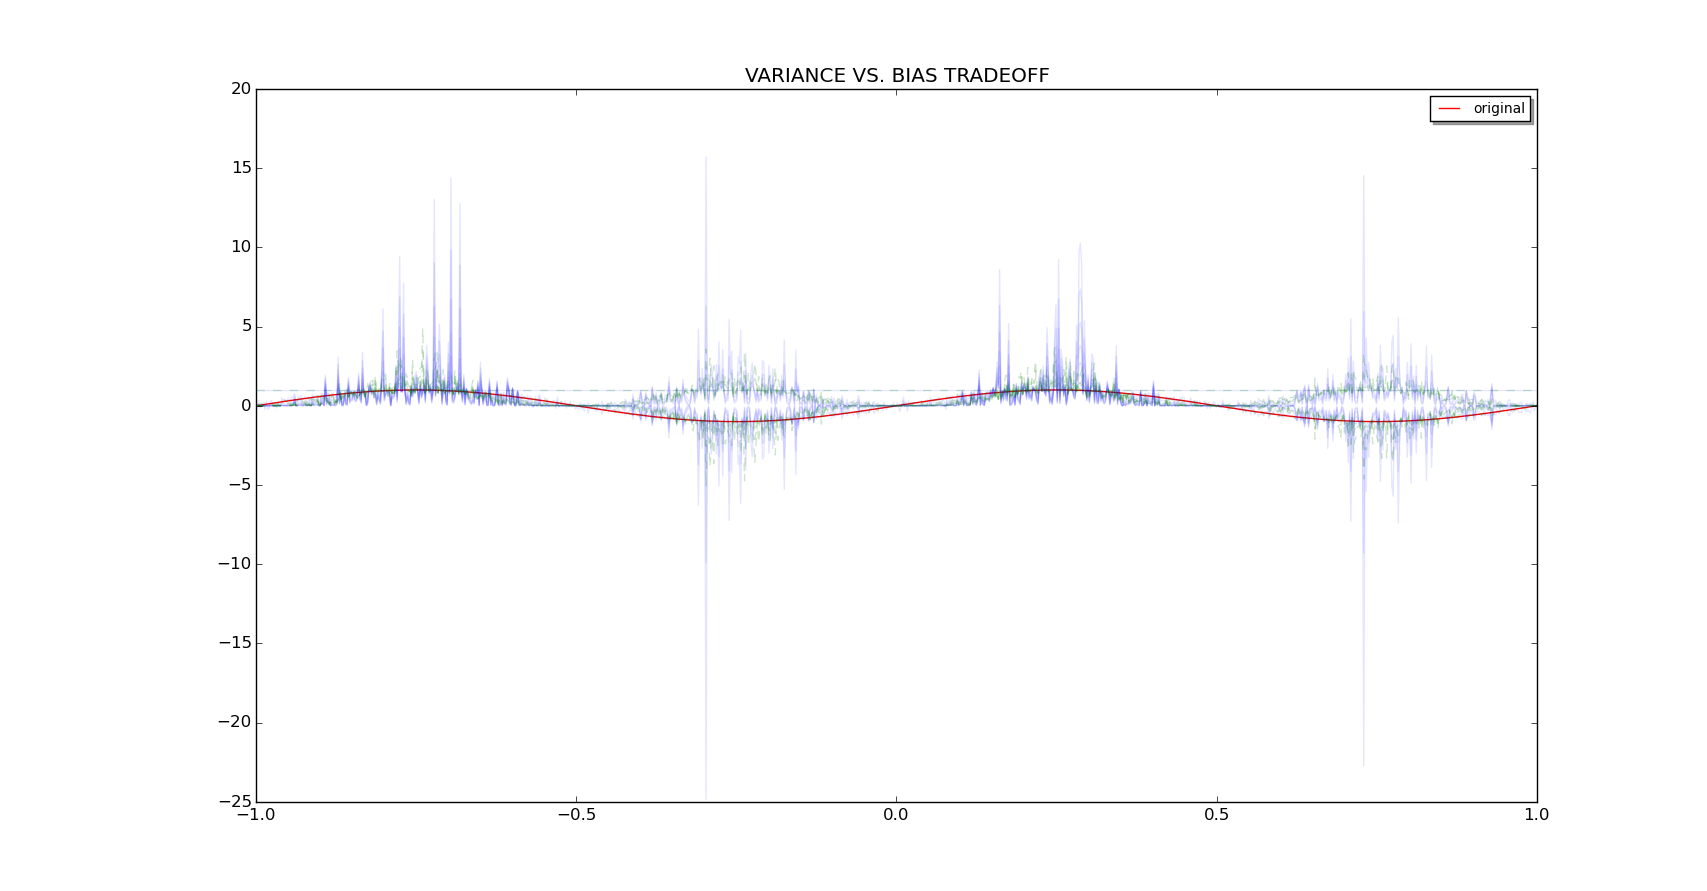
\includegraphics[width=1.1\textwidth, angle=0]{var_bias.png}
	   \caption{generated example illustrating a case of variance (blue) vs. bias (green) tradeoff}
	   \label{fig2}
         \end{figure}

           

\end{document}




\begin{flushright}
  $\square$\\
\end{flushright}
